\chapter{Introduction}
\label{cha:intro}

\subsection{Background}

This study's purpose originates from a Cybersecurity background, and the need for monitoring of low level systems. 
Reverse engineering and binary analysis are prominent fields of cybersecurity and analyzing the code that is being run directly on the system level has recently gained much more traction. 
This can mostly due to recent ssh backdoor being uncovered \cite{collin_xz_2024} and it's possible high severity. 
Additionally this vulnerability was introduced at an extremely low level - by substituting an indirect function call by the operating system \cite{freund_oss-security_2024}. 
This highlights how a cleverly injected payload can bypass most of the lowest level security checks by making the program vulnerable by injecting malicious content at the linking stage.

The problem this thesis and project aims to provide the answer to is peering into the internal memory of a running process and ascertaining information about how does the actual mapped memory correspond to the parts that were used in process initialization.

\subsection{Significance}

As the \verb|/proc| filesystem provides a very powerful, but immensely low-level access to the processes of the linux system. \cite{kerrisk_proc_2010}
The produced tool that can be used to easily perform a task that would normally be obtained by a chain of command line methods (e.g. dump memory, decompile memory, decompile source, compare) makes the analysis and security assesment of a running process a much easier task. 
Additionally the exploration to determine which signatures can be determined from the running process memory should provide useful insights into what threats may be encountered at such low level and how can one protect against them.

%---------------------------------------------------------------------------

\section{Project Goals}
\label{sec:goals}

\subsection{Research Objectives and Questions}

This project's core objective are
\begin{enumerate}
    \item Gain information on how contents of a \verb|\proc| filesystem interface can be analyzed
    
    \item Create an abstraction over the aforementioned interface as well as the source files that were used to construct the contents of the process memory

    \item Create a tool which using the created abstraction can provide insight and analysis into the running process memory
    
    \item Ensure that the produced tool does not harm the running process and only is used to inspect its contents

\end{enumerate}

During the implementation of the tool and accompanying research the following questions should be answered:

\begin{enumerate}
    \item  how do modern operating systems protect themselves from memory-based attacks
    
    \item  how do the aforementioned memory protections influence the structure of the process memory
    
    \item  how does the modern linking process work and what dangers does it present
    
    \item  How are parts of program source and dependencies translate into the process memory, can this process be influenced and/or decrypted?
\end{enumerate}

%---------------------------------------------------------------------------

\section{Architecture}
\label{sec:architecture}

\subsection{Target}

The tool should target Linux-based systems which provide the \verb|/proc| filesystem interface. 
The primary architecture that the solution should target is x86\_64 based systems.
The tool should be usable as a standalone binary which should provide user with an readable interface that can be navigated.

\subsection{Architecture pattern}

As the app's functionality is dependent on multiple components that depend on each other but can be separated excluding some common communication the service architecture was chosen for the task.
As seen in the service diagram \autoref{fig:modules} the tool should be comprised of three different modules.
The reader module will be the most basic one which will interact with the process and the linked libraries and parse their contents. The Analyzer module will call on the reader module to provide the desired output which it will use to provide insights about the data read. The last module will be responsible for the interaction with the user and should provide a way for the user to interact with the generated insights.

\begin{figure}
    \centering
    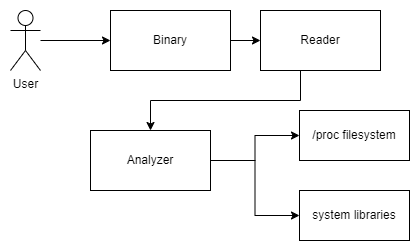
\includegraphics[width=0.5\linewidth]{modules.drawio.png}
    \caption{The user, modules, system and their interaction}
    \label{fig:modules}
\end{figure}

\subsection{Technologies used}

Due to the tool's low level access and safety requirements the Rust programming language seems as the obvious choice as it is a safe systems-level language which also provides a rich typesystem and cargo - rust's integrated build tool and dependency manager. 
Furthermore the language's vast ecosystem of open source packages (also known as crates) the project can make use of many useful tools to ease the development process.
Lastly rust's borrow checker rules \cite{rust_foundation_rust-langrust_2024} enforce program's memory safety which is crucial with interacting within such volatile environments.

\subsection{Limitations}

\begin{enumerate}
    \item The \verb|\proc| filesystem is not part of the UNIX standard \cite{kerrisk_proc_2010} and therefore the tool can be used only on Linux systems which expose it
    \item Different architectures even from the same chip manufacturer can have different instruction sets \cite{intel_corporation_intel_2024}
    \item Sometimes the function and symbol definitions can be mangled or even deliberately erased which limits the tool's usability
    \item Decompilation reverse engineering and binary analysis is a broad subdiscipline of cybersecurity and with scope to broad to fully include in such project
\end{enumerate}
